\documentclass{sig-alternate}
\usepackage{graphicx}
\usepackage{indentfirst}
\usepackage{url}

\begin{document}

\title{PennAnalytics: Real-time Network Traffic Visualization and Analytics}
\subtitle{Dept. of CIS - Senior Design 2013-2014
    \thanks{Advisor: Boon Thau Loo (boonloo@cis.upenn.edu)}}
\author{Patrick Wingo\\ \email{pbwingo@gmail.com}\\ Univ. of Pennsylvania
    \and Aubrey Chase\\ aubchase@seas.upenn.edu\\ Univ. of Pennsylvania
    \and Bill He\\ billshihe@gmail.com\\ Univ. of Pennsylvania
    \and Daniel Ge\\ dange@seas.upenn.edu\\ Univ. of Pennsylvania
    \and Ryan Sasson\\ rsasson@seas.upenn.edu\\ Univ. of Pennsylvania}

\maketitle

\section*{Abstract}

We propose to create a tool to help Penn system administrators better understand
the health and security of their network.  Current networking protocols and
tools present data in a way that is too disaggregated and computer-driven to
understand. We plan to leverage LLDP (Link-Layer Discovery Protocol), SNMP
(Simple Network Management Protocol), as well as NetFlow (packet metadata
inspection) as data sources. In order to more effectively visualize and analyze
the data, we plan to use modern web technologies such as MapReduce for
real-time, large-scale computation, as well as node.js in order to
asynchronously update data between the server processing network data and the
client displaying it.

Our product will differentiate itself on three primary attributes: real-time
analytics enabled through distributed computation, cross-platform compatibility
because of our display through traditional web browsers, as well as focus on
user experience to enhance the analytical abilities of the user. We aim to
create a tool to allow administrators to quickly understand problems at a macro
level, then to easily drill down and display potential problems at the component
level to speed the manual network diagnostics process.

\section*{Glossary}

\textbf{Link Layer Discovery Protocol (LLDP)} is a protocol used to discover the
layout of a network.\cite{ExtremeNetLldp} This protocol allows Ethernet devices
such as routers and bridges to broadcast information about themselves such as
capabilities and neighbors, as well as receive this information from other
devices. Devices broadcast information about themselves, store information they
learn about each other in local databases, and a network management system
accesses this data to build a map of the network topology. The basic unit of
data transmitted by this protocol is a LDP Protocol Data Unit (PDU). A LLDP PDU
consists of a header followed by elements known as TLVs (Type, Length, Value).

\textbf{Netflow} is a protocol used for collecting IP
traffic information.\cite{SolarWindsGuide} On a high level, a flow is a series
of packets that are similar to each other. More specifically, Cisco's Version 5
and Version 9 flow records define a flow by source IP address, destination IP
address, source port number, destination port number, layer 3 protocol type, ToS
byte, and input logical interface. Each flow consists of a flow header, which
contains information such as Netflow version and number of records, and flow
records, which contains information such as source and destination IP, bytes,
and IP protocol. Netflow is sent from routers and switches to a collector
machine where it can be stored, exported, and/or used for analysis.

\textbf{Simple Network Management Protocol (SNMP)} is a protocol that helps
exchange information about a network between the devices in the
network.\cite{ZohoSnmp} The basic setup of an SNMP-managed network consists of
managed devices, agents, and network-management systems. Managed devices run
SNMP agents (software) and store information which can be accessed via SNMP by
the network-management system through a query. It is important to note that SNMP
doesn't define the information that is stored on managed devices and accessed by
the network-management system. Defining the management information is the job of
a database known as the management information base.

\section{Introduction}

Many IT professionals are required to perform analysis of a computer network to
discover information such as percentage of traffic used by certain applications,
which users use the network the most, how usage patterns have changed over time,
and the geographic patterns of network connections. The usage of LLDP, SNMP, and
Netflow data has emerged as a method to perform this analysis and tools such as
NFSen have enabled visualization capabilities by enabling users to look at the
data in a variety of forms such as logs, charts, and graphs.

We believe that existing tools can be improved upon. Log files give extremely
granular detail that provides rich information, but can be overwhelming for a
user. Charts give a high level picture of network statistics, but sacrifice
detail to achieve that simplicity. Existing graph solutions offer a logical and
intuitive way of viewing a network, but fail to incorporate both high level
visualization and low level detail elegantly into one workspace. Furthermore,
existing tools mainly focus on network forensics, but offer little in the way of
incident detection.

We hope to create a network visualization tool that addresses these problems.
Our tool will combine log, chart, and graph visualization methods to
simultaneously offer users a high-level picture of the network and node-level
detail in one workspace. To further enhance the analysis capabilities of users,
we will also incorporate event detection to detect events such as traffic spikes
and security threats to make our system proactive. These capabilities will be
enhanced by performing the analysis in real-time and making our system web-based
and multi-platform.

\section{Related work}

Much software has been written to improve the utilization of NetFlow for network
analysis and visualization, and there are a variety of open- and closed-source
tools available. The same applies for SNMP and LLDP tools. In fact, LLDP is
specifically designed in order to provide information on the topology of a
network, the very thing that we want to first build out, but we find that the
tools are widely disaggregated, and often unintuitive to use. For example, LLDP
is a command line based tool, so that the results output is completely
text-based, and even after reading manuals, it was difficult to understand the
output.

One of the best software packages we found was SolarWinds, a commercial NetFlow
analysis package that breaks down network nodes in tree form, on a map, by CPU
usage, node health, and other metrics.\cite{SolarWinds} We found that it was a
great way to diagnose potential problems with the network, but based on our test
of the free trial, were unable to find out the exact problem. The user interface
was also somewhat confusing: the relationship between different metrics and
graphs was not highlighted. In addition, it appears that LLDP and SNMP were not
incorporated into the solarwinds software; we believe that by integrating
multiple data sets, we can provide a more holistic picture of network health.

Another tool we looked into was Nfsen, an open-source web-based NetFlow
aggregator and analyzer.\cite{NfSen} It took raw NetFlow data from another
open-source tool, nfdump, and visualized it onto a web interface. It solved the
problem of cross-platform visualization, but the graphs are too high-level to be
useful for anything other than knowing there was a problem. We spoke with the
Penn system administrators, and they found nfsen to be useful only in detecting
potential anomalies. From there, they used command tools and sometimes a
multitude of other software platforms in order to understand the problem in
detail. 

Work by Minarik and Dymacek\cite{Minarik08} demonstrated a clear understanding
of the need for system administrators to be able to intuitively understand a
problem using a graph-based, high-level examination, then to drill down on those
nodes and understand statistics for those nodes in order to further
investigate.They even included programmatic DNS, port, and WHOIS lookups in
order to reduce the mechanical work of an analyst, but we found that they did
not use LDDP or SNMP in order to create and understand topology, and their user
interface looked like it could use some improvement as the usage case was not
entirely intuitive.

In terms of work to understand campus wireless networks, we found that Kotz et
al.\cite{Kotz05} used SNMP in order to understand macro-scale campus networks as
wireless was emerging in 2005. Although the research primarily investigated
roaming across the network, which is not entirely relevant to our proposed work,
their method of breaking down traffic across the network using SNMP is relevant.
The researchers polled their access points every 5 minutes using the SNMP
software installed across the network, and got inbound/outbound byte counts as
well as recent MAC addresses. From there, they were able to graph out traffic
over the course of an average day as well as traffic patterns over a long period
of time.

Yin et al.\cite{Yin04} developed a tool called VisFlowConnect which is a
visualization tool that uses a parallel axes representation of Netflow to help
users visualize network traffic. The development of VisFlowConnect was motivated
by the insufficiency of traditional tools to present hostile attack patterns in
an intuitive way for the human mind. VisFlowConnect has various features that
have served as inspiration for our project, including interface views of
different granularity (e.g. global, intra-network) and filtering of data on
various parameters (e.g. protocol, packet-size). However, a shortcoming of
VisFlowConnect is the inability to drill down on the flow data and not only
filter on, but observe information such as protocol and transfer rate. In
addition, we feel that a parallel axes representation of the network can be
somewhat overwhelming and unintuitive and that a graph representation would be
better.

Ball et al.\cite{Ball04} developed a tool called Visual Information Security
Utility for Administration Live (VISUAL) which allows users to see communication
patterns between internal networks and external hosts in a graphical
representation. After surveying IT professionals, Ball, Fink, and North found
that users found it difficult to quickly assess the security state of networks
with text-based tools. They found that with VISUAL, users could develop insights
from the traffic data without any training, demonstrating the power of
visualization tools. VISUAL's main features include markers for external and
internal hosts, color-coded links between external and internal hosts,
interactive filtering, and time lines. Shortcomings of VISUAL that we hope to
address include more proactive displays (e.g. having an internal host flash red
when there is a traffic spike) and processing network data in closer to
real-time.

\section{Proposed work}

\subsection{Overview}

Our objective is to create a system which will be able to analyze network data,
not only in an aggregation fashion, but also in terms of extrapolation. In
addition, we aim to display the network data in a user friendly, yet descriptive
way. The architecture of the application can be broken down into 3 main
components. First, we will have a module that collects and stores data from a
network. Second, this data will be passed to the cloud to be processed and
interpreted. Third, the calculated statistics and information will be displayed
on a clean, interactive web front end. The end goal is to run our system on the
constant stream of information provided by a living network, and we hope to make
the system real-time, or as close to real-time as is possible using our tools.

\begin{figure}[htb!]
    \centering
    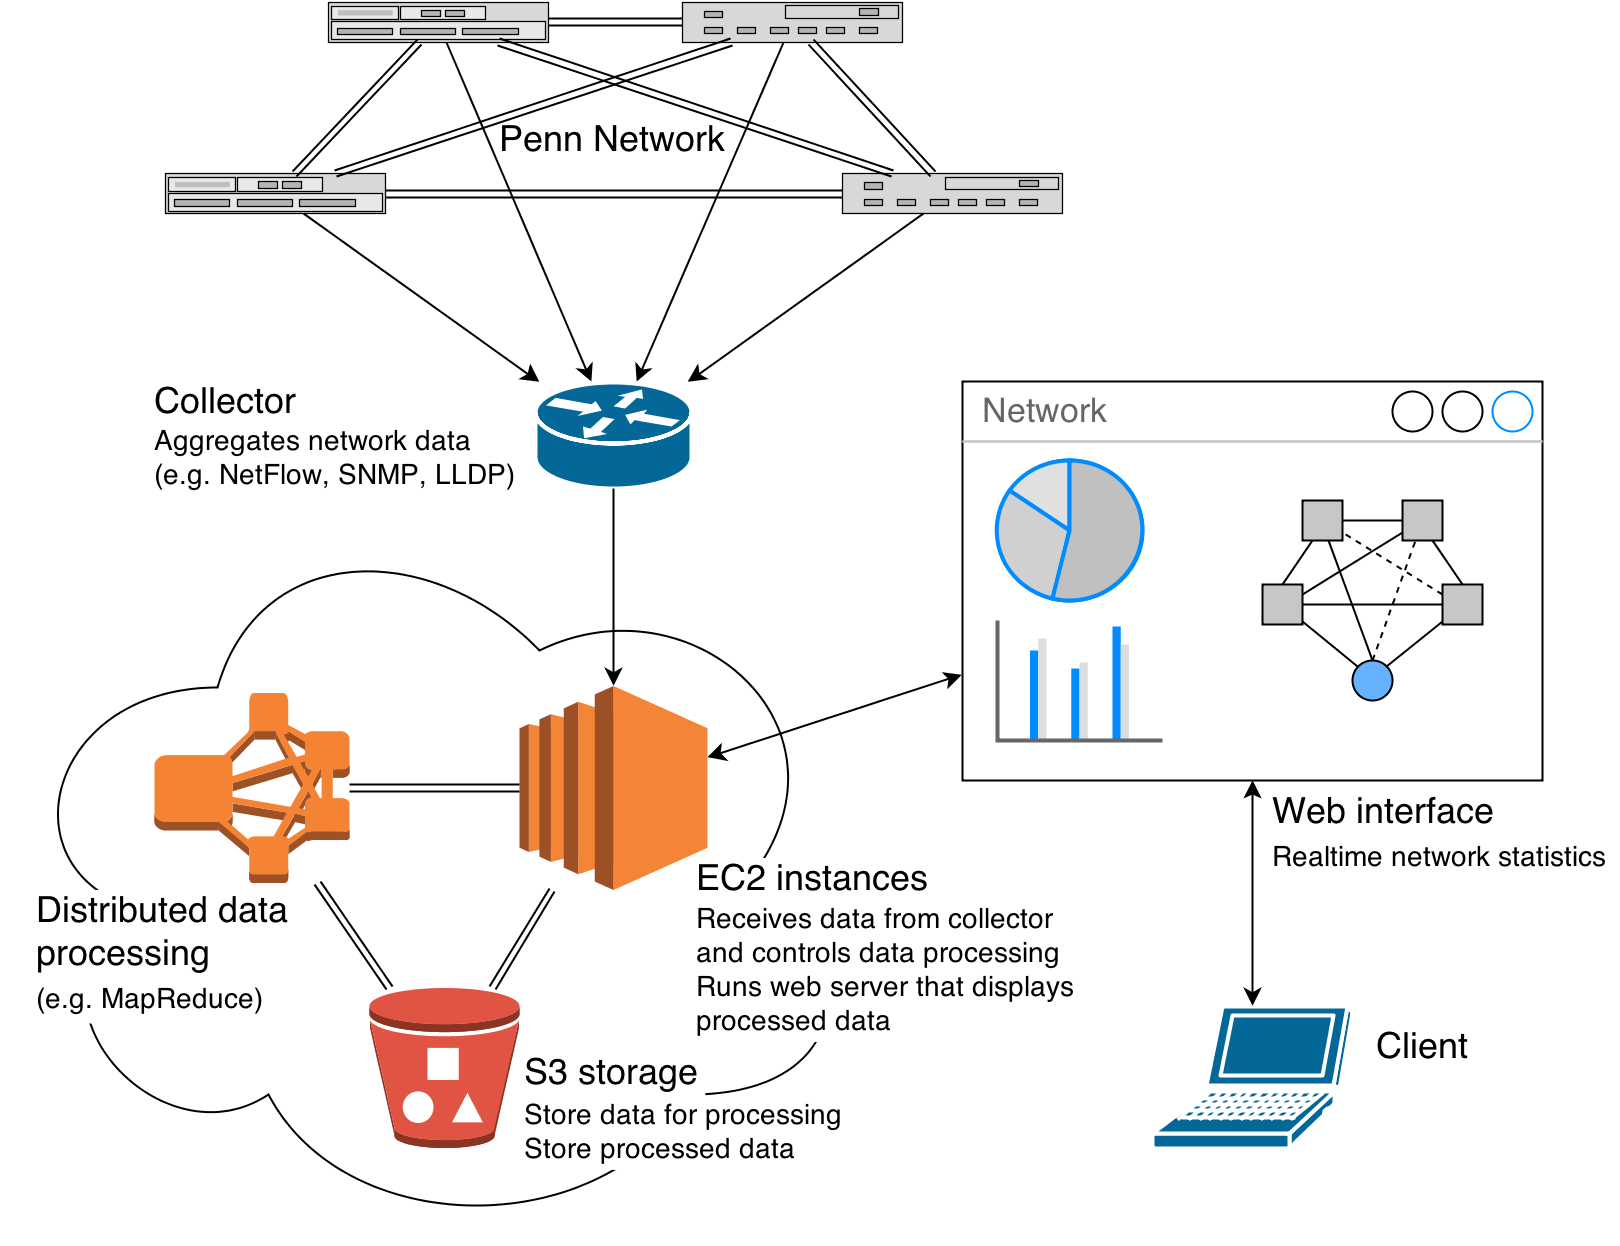
\includegraphics[width=\linewidth]{mockup}
    \caption{Proposed architecture of the project}
    \label{fig:mockup}
\end{figure}

\subsection{Techniques}

We will collect LLDP data, information from SNMP, and hopefully (time
permitting) Netflow data from the Penn Engineering network. This information
must then be transferred to our data processing tools in the cloud. For this to
be possible, we must move the data to a cloud storage base (such as S3 on AWS)
in order to use a horizontally scalable data processing system to extract
aggregate network data.

Once the data has entered the cloud, there are 3 main steps our software will
take to prepare the data for the user. First comes the previously mentioned data
processor. This data processor will take advantage of distributed systems to
make calculations and aggregations quickly. The most well known distributed tool
within our group is Hadoop, so it is the most likely candidate for use in the
analysis. Although Hadoop is a batch process tool, we hope to make real-time,
``streamed'' calculations of the data which we can simulated through frequent
Hadoop jobs. The other option is to replace Hadoop entirely with another tool as
we discuss in the next section.

After that, we must create an index over the calculated data. All this data will
be stored in an easily accessible and queryable database (likely some form of a
SQL database or a distributed SQL database if the data set is large) so the web
frontend server can query it when rendering HTML pages.

Lastly, we must set up a server for the web application front end. For the web
front end we will provide the user a clear and insightful view into the network
data. We will use modern web UI frameworks that leverage HTML, CSS, and
JavaScript so that the application will look consistent among multiple
platforms. The most likely tool we will use for building the front end is the
node.js framework. It is simple, modular, and extremely customizable due to the
possible use of stylesheets.

In order to coordinate the transfer of the data (collector to big data
processor, database to server), it is necessary to use scheduler scripts. For
the initial implementation it would make sense to have a cron job (period job
scheduler) that runs on a EC2 instance that fires up instances for MapReduce
jobs (or another distributed data processing system) and a cron job running on
the network data collector that schedules times for sending network data to a S3
bucket. Later on we look to add synchronization with a fault tolerant job
scheduler if this application scales out to more nodes. Chronos is a possible
tool for distributed and fault tolerant job scheduling.\cite{AirbnbChronos}

\subsection{Anticipated technical challenges}

The first challenge we anticipate is simply the sheer volume of the data we must
aggregate and send to the cloud. This volume could easily reach the scale of
terabytes if collected for long enough. We will devise a way to take this volume
of data and stream it to the processing cluster in the cloud. Transferring this
high volume of data to a cloud service could be potentially costly so we will
need to consider ways to keep this cost low and transfer the data efficiently.
Additionally, If we reach the point where we work with Netflow data we must
address security and privacy concerns with this collection. Most likely we will
need to anonymize the network data before we send it over to the data processor.

Another challenge with the application is the real time implementation; each of
the modules must be synchronized with each other. For example when is there
enough data collected within the collector to be transferred to the Hadoop
stream (or Storm, Spark, etc.)? Or what event will trigger the server to update
the client of state change in the network? Improper implementation can easily
result in modules getting stuck waiting for an update message that never
arrived. Further compounding the difficulty of such an implementation is the
possibility of failure of each modules. Amazon EC2 instances are time shared
virtual machines that run on commodity hardware; we must account for possible
service failure. Additionally it is possible that the collector process could
run out of memory and stop streaming. It is essential to identify these errors
as they occur and to automatically recover from them or to fail gracefully and
not let errors further propagate.

The proposed implementation also has potential performance bottlenecks at
multiple stages of the data transfer. To maintain the real-time nature of the
application, we must address them. One anticipated bottleneck in the current
architecture is the single collector node we have in the Penn Engineering
network. If there is only one node that collects all of the LLDP data within the
Penn network then it will be under much stress due to the high volume. One
potential solution would be to set up a distributed cluster of network data
collectors. Details of this data collection depend on the input of the Penn
Engineering network administrators. Additionally this same node (or nodes) will
be transferring data to AWS over the internet. Transferring a high volume of
data over the internet has the potential to take a very long time. This can be
mitigated by bringing the data processors as close the the collector as
possible. AWS hosts its services in Virginia so the distance is relatively
close. If we want to limit network latency then that would entail setting up a
data processing cluster on campus. This too will have to be discussed with the
network administrators. More details about bottlenecks in the application will
surface as we dive deeper into the implementation.

We are also unsure on what software to use specifically for our cloud analysis.
Within our team, Hadoop is the best known tool at this time. But Hadoop runs
batch processes, and will be harder to stream in a real time environment and
involves large setup and shutdown delays. We have been looking at tools such as
Spark, Storm, and Apache S4 in the hopes of finding a streamable distributed
tool for better real-time updates while still keeping Hadoop's ease of use and
fault tolerance.

A summary of Summingbird, a tool recently manufactured by Twitter for compiling
map reduce problems into either batch or real-time processes, outlines some of
the tradeoffs and problems we will face with this choice. Although Storm
(another of their tools) is faster and streamable, It sacrifices the fault
tolerance of Hadoop's implementation as well as having different problems and
bugs we will have to learn and deal with.\cite{TwitterSummingbird}

Using information from Spark's official webpage\cite{ApacheSpark}, we can see
some touted benefits for their system. They mention that their tool can be up to
100x faster than Hadoop implementations by using in memory computations. This
could lead to its own problems as well though. So, although we are unsure of
which to use, we will most likely start with the system we are most familiar
with (Hadoop) and then prototype the system using the other options so we may
compare the benefits and tradeoffs ourselves. This way, if one does not work, or
any is clearly better than the others, we will be able to identify it, learn it,
and use it.

\subsection{Evaluation criteria}

Our main criteria for evaluation include ease of usability and the ability to
access important information on our software. We want someone with minimal
knowledge of the specific network, or even networks in general, to be able to
use the tool and still understand what we are portraying. We also of course want
the tool to be useful for knowledgeable users. Our program should be able to
display the same information as other applications on the market plus some. In
addition to this, we are also focusing on the visual and interactive components
of the project to try and streamline the user experience.

We also hope that our program will be able to detect and display anomalies to
its users. If we are able to detect attacks or abnormalities in usage in real
time, that alone would constitute a success for the software. The ultimate point
of validation though would be to see Penn's network administrators (or the
administrators of another network) use the software and value it higher than
what they currently use. Our end goal is to create an extensive tool for
displaying detailed and informative network information with a highly user
experience centric front end as we think this technology is currently
unavailable.

\section{Timetable}

While it is difficult to predict with certainty all obstacles we will encounter
in course of the project, we have laid out our preliminary timetable as follows:

\begin{enumerate}
    \item \textsc{October}: Receive LDDP, SNMP Data from Penn. Process it to
        JSON-based graphs.
    \item \textsc{November}: Write LLDP- and SNMP-crunching jobs with MapReduce.
    \item \textsc{December}: Create basic front-end to display node format.
    \item \textsc{January}: Prototype of router node graph and basic statistics
        implemented for Penn.
    \item \textsc{February}: Receive anonymized Netflow data from Penn,
        determine analysis algorithms.
    \item \textsc{March}: Convert analysis algorithms into MapReduce jobs,
        combine with front-end.
    \item \textsc{April}: Polish and test product, fully integrate with Penn's
        network.
\end{enumerate}

If we progress through the project faster than we anticipate, we will attempt to
make our reach goal of implementing algorithms to alert users of anomalous
network activity.

\bibliographystyle{plain}
\bibliography{sources}

\nocite{*}

\end{document}
